%%
% The BIThesis Template for Bachelor Graduation Thesis
%
% 北京理工大学毕业设计(论文)第一章节 —— 使用 XeLaTeX 编译
%
% Copyright 2020 Spencer Woo
%
% This work may be distributed and/or modified under the
% conditions of the LaTeX Project Public License, either version 1.3
% of this license or (at your option) any later version.
% The latest version of this license is in
%   http://www.latex-project.org/lppl.txt
% and version 1.3 or later is part of all distributions of LaTeX
% version 2005/12/01 or later.
%
% This work has the LPPL maintenance status `maintained'.
%
% The Current Maintainer of this work is Spencer Woo.
%
% 第一章节

\chapter{特征构建与预处理}

特征的选择与构建基本上是整个推荐系统的核心所在,也是这个项目中最为复杂的部分,在项目特征的选择上,我们进行了很多的探索,接下来将一一介绍我们的工作。

\section{特征分析}

首先最简单的特征构建方法就是按照经验公式直接将学生的各项指标换算成评分来作为训练数据进行推荐,甚至于可以直接按照分数高低进行推荐,这种方法也是本科生奖学金评选经常使用的一种方法,那么在这个系统中,由于缺少对应研究生已有的经验公式,所以我没有对这部分内容进行实验,而是选择了其它方法。

对于奖学金推荐系统而言,因为推荐使用的特征是多维度的,包括论文、竞赛等诸多部分,所以我选择单独对每种类型的特征进行考虑,由于对应一个学生而言,他可能在一篇论文中有不同的作者等级,发表的论文会有不同的期刊(会议)等级,所以这些都应当作为特征构建中的评价指标,除此以外还应当考虑一个极其重要的问题即为一个学生可能有多篇论文的情况存在,而且这种现象确实已经在系统中出现,在系统中有的学生论文数量达到了3篇,更有甚者在荣誉称号一个单项上就存在7项之多,如何对其进行特征构建就成为了一个棘手的工作,如果要囊括所有学生的记录的话,那么这个特征矩阵将及其庞大,因为对应绝大部分学生来说,在某个单项(论文等)只有一项纪录,而要表示完整的单项需要的特征向量维度较高,如果只考虑竞赛一项按单人最大数量来算,那么只竞赛的表示就至少有7*n(n代表对每个记录选择的特征维数,如论文中的期刊等级以及作者排序等)个维度,所以最后我产生了两种思路,第一种思路是尽可能多的保留各单项信息,每个单项最多选取3个有价值的记录构成特征向量,或者将一个单项的所有信息累加,用公式换算为得分或者对单项信息进行无监督的聚类,将聚类标签作为特征输入推荐算法进行训练。

以上是产生的两种思路,我主要实验了第一种思路,也就是按单项最大个数对记录进行保留,但是我并没有选择简单的对特征进行筛选后直接构建特征向量,而是同时对特征使用聚类的方法以期减少特征的数量以及训练的复杂度。在这里以论文的特征向量构建为例展开分析。

以论文的特征向量构建为例,论文的特征向量主要包括论文刊载的期刊(会议)等级以及学生的作者排序,这两个数据是我们已有的,但是在给定我们的excel文件中,可以看到其他还存在一些额外的信息,比如论文期刊层次的中科院JCR分区大类、中科院JCR分区小类,以及论文他引情况等,至于为什么没有选择剩下的这3个特征进行构建,是因为对于绝大部分论文而言,前两个特征已经足够进行评级并且剩下的3个特征存在的问题分别是JCR分区大类和分区小类没有包括部分国际期刊的分类而完全归于其他分区,导致对部分国际、国内和部分国际、国内会议的区分不够明确,他引情况的问题是他引情况可能随时间变化较大,如较早发表的论文的引用数量较多,而较晚发表的论文可能引用数量不足或根本为0,同时如何获取论文引用数量也是一个很困难的现实,因为我一开始曾经考虑对知网信息进行爬取获得论文的关键词、摘要等按照中文NLP方法以及one-hot编码对论文内容进行简单分类,但是一方面知网有完整的反爬机制除此以外对知网内容进行爬取可能会导致学校IP被暂时封禁,所以最终放弃了这种想法。但是我们选择了使用聚类的方法对论文数据进行处理,接下来将对聚类的实现展开介绍。 

\section{聚类方法}

\subsection{PCA/TSNE特征降维}

聚类使用的主要方法均为无监督聚类,以典型的KMeans方法为例,我们首先对论文数据进行了清洗,并且保留了聚类所用到的两个特征--论文作者排序以及期刊(会议)等级,并且使用TSNE以及PCA两种方法对数据进行了主成分分析、降维以及可视化处理,同时我们使用了one-hot encoding以及label encoding两种方法将文字特征转化为数值特征,理论上而言期刊(会议)等级和作者排序均存在大小关系,所以我们构建的label encoding也是以高等级期刊、高作者排序对应数值低而进行,因此我们自主设定了排序等级,以期刊(会议)等级的label encoding为例:





由上可知期刊(会议)等级排序共8类,所以我们对其进行了一一映射,同时也可以对其进行one-hot encoding,对one-hot encoding后的样本进行TSNE可视化以及主成分分析后的结果如图\ref{TSNE-PCA-one-hot}所示:
\begin{figure}[htb]
    \vspace{13pt} % 调整图片与上文的垂直距离
    \centering
    \begin{minipage}[htb]{0.5\textwidth}
    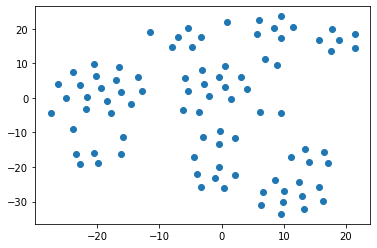
\includegraphics[width=0.4\textwidth]{images/TSNE-one-hot.png}
    \caption{TSNE}
    \end{minipage}
    % \hspace{0.5in}
    \begin{minipage}[htb]{0.5\textwidth}
    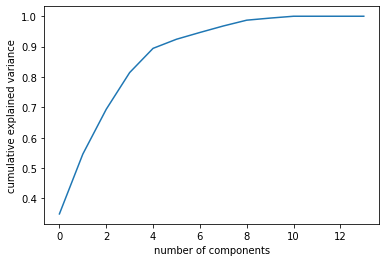
\includegraphics[width=0.4\textwidth]{images/PCA-one-hot.png}
    \caption{PCA}
    \end{minipage}
    \caption{one-hot 编码的TSNE与PCA可视化结果}\label{TSNE-PCA-one-hot} % label 用来在文中索引
  \end{figure}
  




可见主成分在6~8左右(one-hot后的特征向量)对原始特征的还原度较好,在这里可以选择对主成分进行提取;而TSNE的可视化结果则显示样本呈现某种特殊的分布规律,初步验证数据呈现规律分布可以进行聚类。

\subsection{K-Means 聚类}

接下来我首先进行的是使用KMeans方法聚类,根据KMeans的官方文档,对类别特征最好进行one-hot encoding后去除自身的欧几里得距离特征进行聚类更为合适,虽然KMeans对噪声敏感而且初始点的选择可能会影响聚类效果,但KMeans作为一种容易理解简单易懂而且执行速度较快的聚类算法在这种小量数据集上可以有较好的表现,所以我首先选择了KMeans对其进行聚类。由于KMeans要手动选取聚类类数k,所以我首先进行了k=5的聚类,效果虽然不太理想但是证明了KMeans在这个数据集是有效的,接着我对KMeans的聚类结果进行了可视化展示,分别展示了聚类不同类中数据个数以及PCA主成分分析后提取的主成分分布图,结果如下:
\begin{figure}[htb]
    \vspace{13pt} % 调整图片与上文的垂直距离
    \centering
    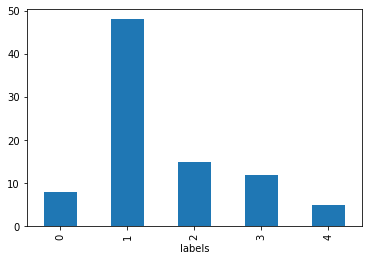
\includegraphics[width=0.4\textwidth]{images/Kmeans-5-label-distribution-label-encoding.png}
    \caption{TSNE}
    \hspace{0.5in}
    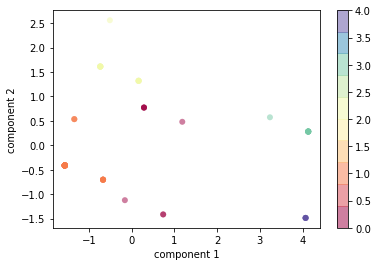
\includegraphics[width=0.4\textwidth]{images/Kmeans-5-PCA-label-encoding.png}
    \caption{PCA}
    \caption{one-hot 编码的TSNE与PCA可视化结果}\label{} % label 用来在文中索引
  \end{figure}


以上左图展示了聚类个数以及聚类的标签之间的关系,右图是PCA的主成分分布情况,从图中来看label中有一个类的数量极多,这个类根据后续的查询也是所有论文中最多的两个成分组成的类,分别是第一作者以及国际会议。

接着我对KMeans进行了优化,主要的优化为以不同的k值进行实验并评价聚类效果,对于聚类效果的评价,我选用的是轮廓系数(silhouette score)和Calinski-Harabasz系数。轮廓系数取值在[-1,1]之间,接近0表示重叠的群集,负值通常表示样本分配给错误的聚类,轮廓系数的值大表示同类样本相距近,不同样本相距远,聚类效果较好;c-h系数主要作用是计算同一类别内部的协方差大小衡量类内的相似性,类内数据的协方差越小越好,类间的协方差越大越好,对于C-H系数而言C-H系数值越高说明聚类的区分度越高。那么我通过这两个指标可视化输出不同k值的系数变化曲线来确定k的最优值。结果如下:



可以看到k=7左右的聚类效果较好,那么在这样的情况下我们考虑使用其它方法进行聚类并评价聚类效果选择最优算法进行聚类,选择的其他算法包括谱聚类以及HDBSCAN。

\subsection{HDBSCAN 聚类}

为了实现自动化的聚类个数n选择,我使用了HDBSCAN进行实验,在HDBSCAN的可视化工作上我生成了HDBSCAN的集群层次结构、生成的提取簇以及压缩聚类树,聚类的效果如下:



可以看到虽然HDBSCAN的效果不甚理想,主要原因是由于HDBSCAN本身是对平面上的数据进行分类,对于大量数据重合的情况分类效果尤其是提取簇和压缩树的效果不明显,但是HDBSCAN也将聚类簇数设置为6,如果再加上label为-1的列(对于HDBSCAN不属于任何聚类簇的标签)那么簇数为7,与KMeans的效果相同,再一次印证了k=7是较优结果。

\subsection{谱聚类}

除此以外我们也使用了谱聚类对聚类结果进行测试,谱聚类同样使用了轮廓系数以及Calinski-Harabasz系数对不同的聚类簇数进行测试,同时也对gamma值进行了调参,gamma是谱聚类算法核函数参数,可视化输出效果如下:



同样可以看到在7-1的组合左右谱聚类的轮廓系数达到最优,但是值得注意的是C-H系数呈现下降的态势,但是总体而言最终还是选择k=7,gamma=1进行聚类较为合适。

\section{特征构建总结}

其他的方法包括单独构建特征,不通过聚类的方法对特征进行one-hot encoding或label encoding直接作为数据特征进行训练或者将聚类结果作为特征而删除所有单独特征节省特征矩阵的长度,但是以上方法由于时间原因未能尝试,尤其是将聚类结果作为全部特征的特征构建也不失为一个构建模型好的选择,这样的方法更适合与对推荐模型进行融合。

除此以外可以考虑的方法还有对连续特征离散化,比如将成绩将成绩分段统计作为特征进行训练。这样可以避免连续取值需要归一化的问题,并且可以更清晰的对分数分布等特征在模型中的作用进行统计。

\section{csv生成}

在生成csv的过程中我们也充分考虑了论文等级论文期刊存在的偏序关系,以论文的排序举例,首先是按照用户的user\_id进行排序,接下来按照论文层次进行排序,然后按照论文的作者等级进行排序,最后按照论文的期刊等级排序,在这样的排序条件下,虽然可能出现一个人有多个论文的情况,但是可以保证所有的数据都是以特定规则排列而不是无规则排列,这样在模型训练过程中会更为准确。除此以外对于论文等特征我们也统计了论文数量作为特征之一,而且在实验中证明论文数量也是影响奖学金评定的重要因素。

在特征设计的过程中为了将one-hot后离散的稀疏特征进行降维可以选择多种方法,其中比较典型的方法为借用word2Vec的思想加入embedding层进行嵌入训练将特征转化为低维稠密且元素不为0的特征,或者通过决策树等方式对特征进行降维处理。我们在DeepFM中验证了前一种方法,并且使用了XGBoost验证了第二种方法。

% 这里插入一个参考文献,仅作参考
